\chapter{Utilerias HTML}

\section{zend\_django.templatetags.html\_helpers}

\subsection{Funciones}

\begin{lstlisting}[language=Python]
get_apps() : list
\end{lstlisting}

\subsection{Inclusion Tags}

\begin{lstlisting}[language=Python]


generate_get_css_apps() : {'apps': list_obj}
generate_get_js_apps() : {'apps': list_obj}
requiere_ui_css(context) : {'apps': ['jquery-ui']} | {}
requiere_ui_js(context) : {'apps': ['jquery-ui.min', 'datepicker-es'], 'req_ui': True} | {}

context.request.META[`"HTTP_USER_AGENT"]
\end{lstlisting}

\section{zend\_django.templatetags.op\_helpers}

\subsection{CRUDs}

\begin{itemize}
	\item create
	\item create\_f
	\item read
	\item update
	\item delete
	\item list
\end{itemize}

\subsection{Actions}

\begin{itemize}
	\item save
	\item ok
	\item cancel
	\item send\_mail
	\item call
	\item send\_whatsapp
	\item reset\_password
\end{itemize}

\subsection{Simple Tags}

\begin{lstlisting}[language=Python]


crud_icon(operation): string
crud_label(operation): string
crud_smart_button(operation): string

action_icon(action): string
action_label(action): string
action_smart_button(operation): string
\end{lstlisting}

\section{html\_struct.html}

\begin{tabular}{|l|l|}
	\hline
	Llamada como & zend\_django/html/html\_struct.html \\
	\hline
	Carga & html\_helpers \\
	& op\_helpers \\
	& parametros\_helpers \\
	\hline
\end{tabular}

\begin{figure}[H]
	\centering
	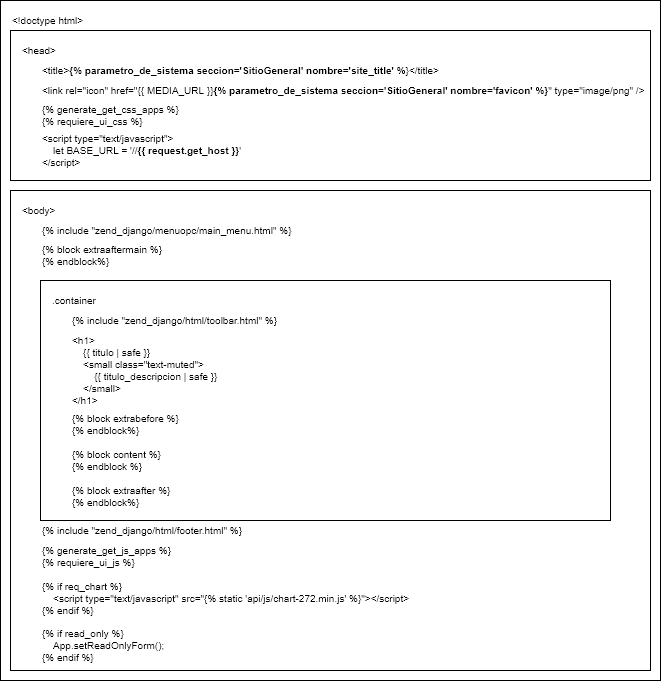
\includegraphics[scale=0.65]{./diagram/html_struct_html}
	\caption{html\_struct.html}
\end{figure}

\section{toolbar.html}

\begin{lstlisting}[language=Python]
toolbar = [
{'type': 'rlink',       'label': 'Etiqueta',    'url': 'http://...'},
{'type': 'link',        'label': 'Etiqueta',    'view': 'NombreVista'},
{'type': 'link_pk',     'label': 'Etiqueta',    'view': 'NombreVista',  pk: 'Valor'},
{'type': 'link_pk_del', 'label': 'Etiqueta',    'view': 'NombreVista',  pk: 'Valor'},
{'type': 'button',      'label': 'Etiqueta',    'onclick': 'CodigoJS'},
{'type': 'search'},
]
\end{lstlisting}

\section{form.html}

\begin{tabular}{|l|l|}
	\hline
	Llamada como & zend\_django/html/form.html \\
	\hline
	Extiende & zend\_django/html/html\_struct.html \\
	\hline
	Carga & crispy\_forms\_tags \\
	& op\_helpers \\
	\hline
\end{tabular}

\begin{lstlisting}
forms = {
	'top': [{'title':'XXXX', 'form': form_object}, ...],
	'left': [...],
	'right': [...],
	'bottom': [...],
}
\end{lstlisting}

\begin{figure}
	\centering
	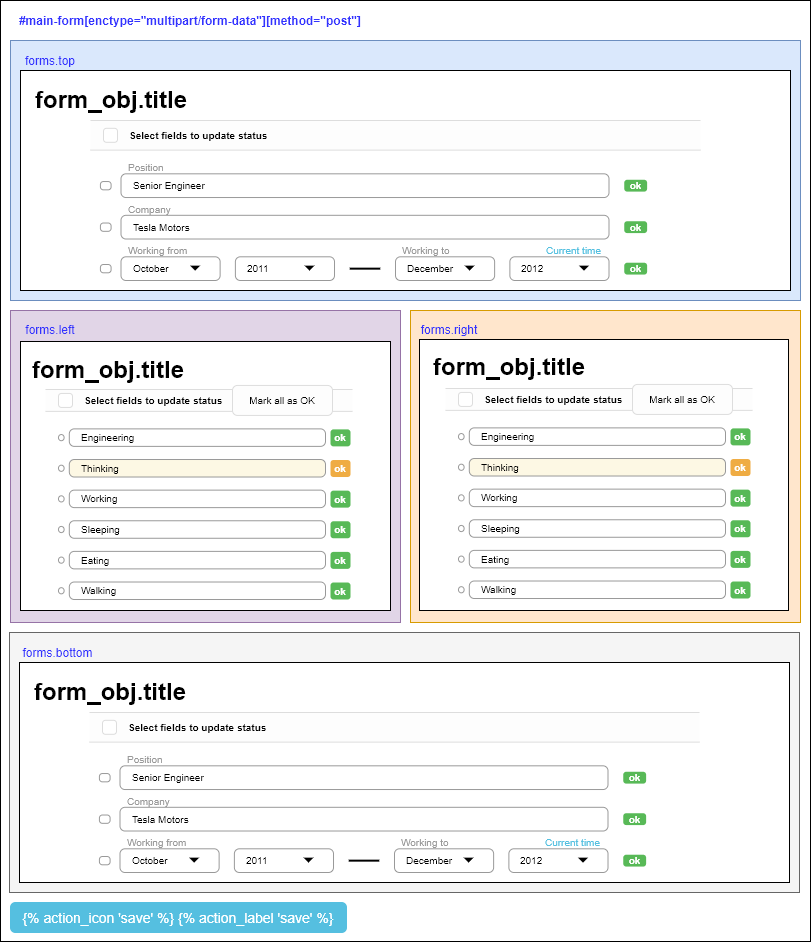
\includegraphics[scale=0.65]{./diagram/forms_html}
	\caption{forms.html}
\end{figure}
